\chapter{Mixture models and EM}
\label{chap:EM}

\section{Introduction}
If we define a joint distribution over observed and latent variables,the corresponding distribution of the observed variables alone is marginalization.Mixture distributions can be interpreted in terms of discrete latent variables.As well as providing framework for building more complex probability distributions,mixture models can also be used to cluster data.

\section{$K$-means Clusetering}
\subsection{representation}
Suppose we have a data set $\{\vec{x}_1,...,\vec{x}_N\}$ consisting of $N$ observations of a random $D$-dimensional Euclidean variable $\vec{x}$.Our goal is to partition the data set into some number $K$ of clusters.First introduce a set of $D$-dimensional vectors $\vec{\mu}_k$,where $k=1,...,K$,in which $\vec{\mu}_k$ is a prototype associated with the $k^{th}$ cluster,representing the centers of the clusters.

Our goal is then to find an assignment of data points to clusters,as well as a set of vectors $\{\vec{\mu}_k\}$,such that the sum of squares of the distances of each data point to its closest vector $\vec{\mu}_k$,is a minimum.

A corresponding set of binary indicator variables $r_{nk}\in \{0,1\}$,describing which of the $K$ clusters the data point $\vec{x}_n$ is assigned to,so that if data point $\vec{x}_n$ is assigned to cluster $k$ then $r_{nk}=1$,and $r_{nj}=0$ for $j\neq k$.This is the 1-of-$K$ coding scheme.


\subsection{evaluation}
Define the objective function,sometimes called a \textbf{distortion measure} as
\begin{equation}
J=\sum_{n=1}^{N}\sum_{k=1}^{K}r_{nk}\parallel \vec{x}_n-\vec{\mu}_k\parallel^2
\end{equation}

\subsection{optimization}
Our goal is to find value for the $\{r_{nk}\}$ and the $\{\vec{\mu}_k\}$ so as to minimize $J$.We can do this through an iterative procedure in which each iteration involves two successive steps corresponding to successive optimizations with respect to the $r_{nk}$ and the $\vec{\mu}_k$,which can be interpreted as parameters of each cluster's probability distribution.

Consider first the determination of the $r_{nk}$,which can be interpreted as likelihood function of each cluster.We simply assign the $n^{th}$ data point to the closest cluster centre.
\begin{equation}
r_{nk} = \begin{cases}
1,\text{if }k=\arg\min_j\parallel \vec{x}_n-\vec{\mu}_j\parallel^2 \\
0,\text{otherwise} \\
\end{cases}
\end{equation}
Note that
\begin{align}
\arg\min_j\parallel \vec{x}_n-\vec{\mu}_j\parallel^2
&= \arg\min_j(\parallel \vec{x}_n\parallel ^2-2\parallel \vec{x}_n\parallel\parallel \vec{\mu}_j\parallel + \parallel\vec{\mu}_j\parallel^2)  \\
&=\arg\min_j(-2\parallel \vec{x}_n\parallel\parallel \vec{\mu}_j\parallel + \parallel\vec{\mu}_j\parallel^2)   \\
&=\arg\max_j(\vec{x}_n^T\vec{\mu}_j-\dfrac{\vec{\mu}_j^T\vec{\mu}_j}{2})
\end{align}
Now consider the optimization of the $\vec{\mu}_k$ with the $_{nk}$ held fixed.Setting the objective function $J$'s derivative with respect to $\vec{\mu}_k$ to zero giving:
\begin{align}
	\nabla_{\vec{\mu}_k} J
	&=2\sum_{n=1}^{N}r_{nk}(\vec{x}_n-\vec{\mu}_k)=0 \\
	\Rightarrow 
	\vec{\mu}_k &=\dfrac{\sum_n{r_{nk}\vec{x}_n}}{\sum_n{r_{nk}}} \\
	\Rightarrow
	\vec{\mu}_k^T &= \dfrac{\sum_n{r_{nk}\vec{x}_n^T}}{\sum_n{r_{nk}}}
\end{align}
which can be vectorized when implementing.

\begin{algorithm}[H]
	\caption{{\sc K-means} coordinate descent}
	\label{algo:K-means}
	%\DontPrintSemicolon % Some LaTeX compilers require you to use \dontprintsemicolon instead 
	\KwIn{A set $\vec{X} = \{\vec{x}_1, \vec{x}_2, \ldots, \vec{x}_N\}$}
	\KwOut{$\{r_{nk}\}$ and the $\{\vec{\mu}_k\}$ such that $J$ is minimized.}
	 initialize $\vec{\mu}_k$\;
	\Repeat{converged}{
		%$C \gets \emptyset$\;
		E(expectation).Minimize $J$ with respect to the $r_{nk}$.$r_{nk} = \begin{cases}
			1,\text{if $k=\arg\min_j\parallel \vec{x}_n-\vec{\mu}_j\parallel^2$ } \\
			0,\text{otherwise} \\
		\end{cases}$,keeping $\vec{\mu}_k$ fixed \;
		M(maximization).Minimize $J$ with respect to the $\vec{\mu}_k$:
		$\vec{\mu}_k=\sum_n r_{nk}\vec{x}_n \over \sum_n r_{nk}$,keeping $r_{nk}$ fixed.\;
 	}

\end{algorithm}

The objective may converge to a local rather than global minimum(MacQueen 1967).

Derive an on-line stochastic rather than the batch version of $K$-means,by applying Robbin-Monro procedure :
\begin{align}
\vec{\mu}_k^{new} = 
\vec{\mu}_k^{old} + \eta_n(\vec{x}_n-\vec{\mu}_k^{old})
\end{align}
where $\eta_n$ is the learning rate parameter,which is typically made to decrease monotonically as more data points are considered.

Generalize the $K$-means algorithm,introducing a general dissimilarity measure $\nu(\vec{x},\vec{x}')$
\begin{align}
\hat{J} = \sum_{n=1}^{N}\sum_{k=1}^{K}r_{nk}\nu(\vec{x}_n,\vec{\mu}_k)
\end{align}
which gives the \textbf{$K$-medoids} algorithm.The computation cost of E step is $O(KN)$.The M step is potentially more complex.So it is common to restrict each cluster prototype to be equal to one of the data vectors assigned to that cluster,requiring $O(N_k^2)$ evaluations of $\nu(\cdot,\cdot)$.

\section{Mixtures of Gaussians}
\subsection{representation}
The Gaussian mixture distribution can be written as a linear superposition of Gaussians in the form
\begin{align}\label{def:Gaussian mixture}
p(\vec{x}) =
\sum_{k=1}^{K}\pi_k\mathcal{N}(\vec{x}|\vec{\mu}_k,\vec{\Sigma}_k)
\end{align}
Introduce a $K$-dimensional binary random variable $\vec{z}$ having a $1$-of-$K$ representation.
\begin{align}
z_k &\in \{ 0,1\} \\
\sum_k z_k &=1
\end{align}
The marginal distribution over $\vec{z}$ is specified in terms of the mixing coefficients $\pi_k$,such that
\begin{align}
p(z_k=1) = \pi_k
\end{align}
where the parameters $\{ \pi_k\}$ must satisfy
\begin{align}
0 \leq &\pi_k \leq 1\\
\sum_{k=1}^{K} &\pi_k = 1
\end{align}
Write this distribution in the form
\begin{align}
p(\vec{z}) = \prod_{k=1}^{K}\pi_k^{z_k}
\end{align}
The conditional distribution of $\vec{x}$ given a particular value for $\vec{z}$ is a Gaussian:
\begin{align}
p(\vec{x}|z_k=1) &= \mathcal{N}(\vec{x}|\vec{\mu}_k,\vec{\Sigma}_k) \\
p(\vec{x}|\vec{z}) 
&=\prod_{k=1}^{K}\mathcal{N}(\vec{x}|\vec{\mu}_k,\vec{\Sigma}_k)^{z_k}
\end{align}
The joint distribution is given by $p(\vec{z})p(\vec{x}|\vec{z})$,and the marginal distribution of $\vec{x}$ is obtained by summing the joint distribution over states of $\vec{z}$:
\begin{align}
p(\vec{x}) = \sum_{\vec{z}}{p(\vec{z})p(\vec{x}|\vec{z})} =
\sum_{k=1}^{K}\pi_k\mathcal{N}(\vec{x}|\vec{\mu}_k,\vec{\Sigma}_k)
\end{align}
which is a Gaussian mixture \ref{def:Gaussian mixture} .

The conditional probability of $\vec{z}$ given $\vec{x}$ can be evaluated by Bayes' theorem
\begin{align}
\label{eqn:responsibility}
\gamma(z_k)\equiv p(z_k=1|\vec{x}) 
&=\dfrac{p(z_k=1)p(\vec{x}|z_k=1)} {\sum_{j=1}^{K}p(z_j=1)p(\vec{x}|z_j=1)} \\
&=\dfrac{\pi_k \mathcal{N}(\vec{x}|\vec{\mu}_k,\vec{\Sigma}_k)}  
	{\sum_{j=1}^{K}\pi_j\mathcal{N}(\vec{x}|\vec{\mu}_j,\vec{\Sigma}_j)}
\end{align}
We shall view $\pi_k$ as the prior probability of $z_k=1$,and the quantity $\gamma(z_k)$ as the corresponding posterior.$\gamma(z_k)$ can also be viewed as the \textbf{responsibility} that component $k$ takes for 'explaining' the observation $\vec{x}$.

\subsection{Maximum likelihood}
Assuming that the data points are drawn independently from the same distribution(i.i.d),the log of the likelihood function is given by
\begin{align}\label{eqn:Gaussian mixture log likelihood}
\ln(p(\vec{X}|\vec{\pi},\vec{\mu},\vec{\Sigma})) =
\sum_{n=1}^{N}\ln\{\sum_{k=1}^{K}\pi_k\mathcal{N}(\vec{x}_n|\vec{\mu}_k,\vec{\Sigma}_k) \}
\end{align}

It is worth emphasizing that there are significant problems associated with the maximum likelihood framework applied to GMM,due to the presence of \textbf{singularities}.If one of the components of the mixture model 'collapse' onto a specific data point($\sigma_j\rightarrow 0$),the log likelihood function will go to infinity.These singularities provide another example of severe over-fitting of maximum likelihood approach.A further issue is \textbf{identifiability}(Casella and Berger,2002),which is that a $K$-component mixture results in $K!$ equivalent solutions.

\subsection{EM for Gaussian mixtures}
An elegant and powerful method for finding the maximum likelihood solutions for models with latent variables is called the \textbf{expectation-maximization},or EM algorithm.

Begin by writing down the conditions that must be satisfied at a maximum of the likelihood function.Setting the derivatives of $\ln p(\vec{X}|\vec{\pi},\vec{\mu},\vec{\Sigma})$ \ref{eqn:Gaussian mixture log likelihood} with respect to the means $\vec{\mu}_k$ of the Gaussian components to zero,we obtain
\begin{align}
\because 0&=-\sum_{n=1}^{N}\dfrac{\pi_k\mathcal{N}(\vec{x}_n|\vec{\mu}_k,\vec{\Sigma}_k)}
{\sum_{j=1}^{K}\pi_j\mathcal{N}(\vec{x}_n|\vec{\mu}_j,\vec{\Sigma}_j)}
\vec{\Sigma}_k^{-1}(\vec{x}_n-\vec{\mu}_k) \\
\therefore 0&=-\sum_{n=1}^{N}\gamma(z_{nk})(\vec{x}_n-\vec{\mu}_k) \\
\because
N_k&=\sum_{n=1}^{N}\gamma(z_{nk}) \\
\therefore \vec{\mu}_k&=\dfrac{1}{N_k}\sum_{n=1}^{N}\gamma(z_{nk})\vec{x}_n \\
\end{align}
where we have made use of $\dfrac{de^x}{dx}=e^x$ and \ref{eqn:multivariate Gaussian}.We can interpret $N_k$ as the effective number of points assigned to cluster $k$.

Now set the derivative of $\ln(\vec{X}|\vec{\pi},\vec{\mu},\vec{\Sigma})$ with respect to $\vec{\Sigma}_k$ to zero:
\begin{align}
\dfrac{\partial\ln p(\vec{X}|\vec{\pi},\vec{\mu},\vec{\Sigma})}{\partial\vec{\Sigma}_k} 
&=\sum_{n=1}^{N}\dfrac{\dfrac{\partial(\pi_k\mathcal{N}(\vec{x}_n|\vec{\mu}_k,\vec{\Sigma}_k))}{\partial\vec{\Sigma}_k}}
{\sum_{j=1}^{K}\pi_k\mathcal{N}(\vec{x}_n|\vec{\mu}_k,\vec{\Sigma}_k)}\\
\because
 \dfrac{\partial \ln y}{\partial x} &= \dfrac{1}{y}\dfrac{\partial y}{\partial x} \\
\therefore \dfrac{\partial y}{\partial x} &= y\dfrac{\partial\ln y}{\partial x}\\
\because \dfrac{\partial(\pi_k\mathcal{N}(\vec{x}_n|\vec{\mu}_k,\vec{\Sigma}_k))}{\partial\vec{\Sigma}_k} 
&= \pi_k\dfrac{\partial\mathcal{N}(\vec{x}_n|\vec{\mu}_k,\vec{\Sigma}_k)}{\partial\vec{\Sigma}_k}\\
&= \pi_k\mathcal{N}(\vec{x}_n|\vec{\mu}_k,\vec{\Sigma}_k)
\dfrac{\partial\ln\mathcal{N}(\vec{x}_n|\vec{\mu}_k,\vec{\Sigma}_k)}{\partial\vec{\Sigma}_k}\\
\because 
\mathcal{N}(\vec{x}|\vec{\mu},\vec{\Sigma})
&=\dfrac{1}{(2\pi)^{D/2}}\dfrac{1}{\mid \vec{\Sigma}\mid^{1/2}}
\exp\{-\dfrac{1}{2}(\vec{x}-\vec{\mu})^T\vec{\Sigma}^{-1}(\vec{x}-\vec{\mu}) \} \\
\therefore \dfrac{\partial\ln\mathcal{N}(\vec{x}_n|\vec{\mu}_k,\vec{\Sigma}_k)}{\partial\vec{\Sigma}_k}
&=-\dfrac{1}{2}(\dfrac{\ln(\mid\vec{\Sigma}_k)\mid}{\partial\vec{\Sigma}_k}
 +\dfrac{\partial(\vec{x}_n-\vec{\mu}_j)\vec{\Sigma}^{-1}(\vec{x}_n-\vec{\mu}_j)}{\partial\vec{\Sigma}_k}) \\
\because
 \dfrac{\partial det(\vec{X})}{\vec{X}} &=det(\vec{X})(\vec{X}^{-1})^T \\
\dfrac{\partial\vec{a}^T\vec{X}^{-1}\vec{b}}{\partial\vec{X}}
&= -\vec{X}^{-T}\vec{a}\vec{b}^T\vec{X}^{-T} \\
\therefore 
\dfrac{\ln(\mid\vec{\Sigma}_k)\mid}{\partial\vec{\Sigma}_k}
&=\dfrac{\dfrac{\partial\mid\vec{\Sigma}_k\mid}{\partial\vec{\Sigma}_k}}{\mid\vec{\Sigma}_k\mid} =\dfrac{\mid\vec{\Sigma}_k\mid\vec{\Sigma}_k^{-T}}{\mid\vec{\Sigma}_k\mid} =\vec{\Sigma}_k^{-1}\\
\therefore 
\dfrac{\partial\ln\mathcal{N}(\vec{x}_n|\vec{\mu}_k,\vec{\Sigma}_k)}{\partial\vec{\Sigma}_k} 
&=-\dfrac{1}{2}(\vec{\Sigma}_k^{-1}-\vec{\Sigma}_k^{-1}(\vec{x}_n-\vec{\mu}_k)(\vec{x}_n-\vec{\mu}_k)^T\vec{\Sigma}_k^{-1}) \\
\therefore derivative&=\sum_{n=1}^{N}\gamma(z_{nk})(-1/2)[\vec{\Sigma}_k^{-1}-\vec{\Sigma}_k^{-1}(\vec{x}_n-\vec{\mu}_k)(\vec{x}_n-\vec{\mu}_k)^T\vec{\Sigma}_k^{-1}] =0 \\
\therefore \vec{\Sigma}_k&=\dfrac{1}{N_k}\sum_{n=1}^{N}\gamma(z_{nk})(\vec{x}_n-\vec{\mu}_k)(\vec{x}_n-\vec{\mu}_k)^T
\end{align}
where we have made use of \ref{eqn:multivariate Gaussian} and \textbf{The Matrix Cookbook,2012}.

Finally,we maximize $\ln p(\vec{X}|\vec{\pi},\vec{\mu},\vec{\Sigma})$ \ref{eqn:Gaussian mixture log likelihood} with respect to the mixing coefficients $\pi_k$.Achieve this using a Lagrange multiplier
\begin{align}
\ln p(\vec{X}|\vec{\pi},\vec{\mu},\vec{\Sigma}) +\lambda(\sum_{k=1}^{K}\pi_k-1) &=0 \\
\therefore \sum_{n=1}^{N}\dfrac{\mathcal{N}(\vec{x}_n|\vec{\mu}_k,\vec{\Sigma}_k)}
{\sum_{j=1}^{K}\pi_j\mathcal{N}(\vec{x}_n|\vec{\mu}_j,\vec{\Sigma}_j)} +\lambda &= 0
\end{align}
where again we see the appearance of the responsibilities \ref{eqn:responsibility}.If we now multiply both sides by $\pi_k$ and sum over $k$ making use of constraint $\sum_{k=1}^{K}\pi_k = 1$,we find $\lambda = -N$.Then 
\begin{align}
\pi_k = \dfrac{N_k}{N}
\end{align}
There do suggest s ample iterative scheme for finding a solution to the maximum likelihood problem.

\begin{algorithm}[H]
	\caption{EM for Gaussian Mixtures}
	\label{algo:Gaussian Mixtures}
	\DontPrintSemicolon
	\Repeat{\text{convergence of either the parameters or the log likelihood}}{
		1.Initialize the means $\vec{\mu}_k$,covariances $\vec{\Sigma}_k$ and mixing coefficients $\pi_k$,and evaluate the initial value of the log likelihood\;
		2.\textbf{E step}.Evaluate the responsibilities using the current parameter values
		\begin{align}
		\gamma(z_k)\equiv p(z_k=1|\vec{x}) 
		&={p(z_k=1)p(\vec{x}|z_k=1) \over \sum_{j=1}^{K}p(z_j=1)p(\vec{x}|z_j=1)} \\
		&={\pi_k \mathcal{N}(\vec{x}|\vec{\mu}_k,\vec{\Sigma}_k) \over 
		\sum_{j=1}^{K}\pi_j\mathcal{N}(\vec{x}|\vec{\mu}_j,\vec{\Sigma}_j)}
		\end{align} \;
		3. \textbf{M step}. Re-estimate the parameters using the current responsibilities
		\begin{align}
		\vec{\mu}_k^{new} &= \dfrac{1}{N_k}\sum_{n=1}^{N}\gamma(z_{nk})\vec{x}_n \\
		\vec{\Sigma}_k^{new} &=\dfrac{1}{N_k}\sum_{n=1}^{N}\gamma(z_{nk})(\vec{x}_n-\vec{\mu}_k)(\vec{x}_n-\vec{\mu}_k)^T \\
		\pi_k^{new}&= \dfrac{N_k}{N}
		\end{align}\;
		where 
		\begin{align}
		N_k&=\sum_{n=1}^{N}\gamma(z_{nk})
		\end{align}
		4. Evaluate the log likelihood
		\begin{align}
		\ln(p(\vec{X}|\vec{\pi},\vec{\mu},\vec{\Sigma})) =
		\sum_{n=1}^{N}\ln\{\sum_{k=1}^{K}\pi_k\mathcal{N}(\vec{x}_n|\vec{\mu}_k,\vec{\Sigma}_k) \}
		\end{align}\;
	}
\end{algorithm}

\section{Latent Variables View of EM}
\subsection{representation}
We denote the set of all observed data by $\vec{X}$,in which the $n^{th}$ row represents $\vec{x}_n^T$,and denote the set of all latent variables by $\vec{Z}$,with corresponding rows $\vec{z}_n^T$.The set of all model parameters is denoted by $\vec{\theta}$,so the log likelihood function is given by
\begin{align}
\ln p(\vec{X}|\vec{\theta}) &=
\ln\{\sum_{\vec{z}}p(\vec{X},\vec{Z}|\vec{\theta}) \}
\end{align}
Replace the sum over $\vec{Z}$ with an integral for continuous latent variables.

$\{\vec{X},\vec{Z}\}$ is called the \textbf{complete} data set,and $\{\vec{X}\}$ is \textbf{incomplete}.We consider complete-data log likelihood functions' expected value under the posterior distribution of the latent variables,corresponding to the E step.In the subsequent M step,maximize this expectation.The expectation of complete-data log likelihood
\begin{align}
\mathcal{Q}(\vec{\theta},\vec{\theta}^{old}) &=
\sum_{\vec{z}}p(\vec{Z}|\vec{X},\vec{\theta}^{old})\ln p(\vec{X},\vec{Z}|\vec{\theta})
\end{align}
Maximize this
\begin{align}
\vec{\theta}^{new} &=\arg\max\limits_{\vec{\theta}}\mathcal{Q}(\vec{\theta},\vec{\theta}^{old})
\end{align}
\begin{algorithm}[H]
	\label{General EM algorithm}
	\caption{General EM algorithm}
	\DontPrintSemicolon
	\KwIn{$p(\vec{X},\vec{Z}|\vec{\theta})$,$\vec{Z}$}
	\KwOut{output}
	\Repeat{converged}{
		1. Choose an initial setting for the parameters $\vec{\theta}^{old}$.\;
		2. \textbf{E step} Evaluate $p(\vec{Z}|\vec{X},\vec{\theta}^{old})$.\;
		3. \textbf{M step} Evaluate $\vec{\theta}^{new}$ given by
		\begin{align}
		\mathcal{Q}(\vec{\theta},\vec{\theta}^{old}) &=
		\sum_{\vec{z}}p(\vec{Z}|\vec{X},\vec{\theta}^{old})\ln p(\vec{X},\vec{Z}|\vec{\theta})
		\end{align}
		where
		\begin{align}
		\vec{\theta}^{new} &=\arg\max\limits_{\vec{\theta}}\mathcal{Q}(\vec{\theta},\vec{\theta}^{old})
		\end{align} \;
		4. 
		\begin{align}
		\vec{\theta}^{old} \gets \vec{\theta}^{new}
		\end{align}
	}
\end{algorithm}
When finding MAP(maximum posterior) solutions,maximize the quantity $\mathcal{Q}(\vec{\theta},\vec{\theta}^{old})+\ln p(\vec{\theta})$ in M step.

\section{The EM Algorithm in General}
The \textbf{expectation maximization} algorithm,or EM,is a general technique for finding maximum likelihood solutions for probabilistic models having latent variables.

Given the same setting as previous,our goal is to maximize the likelihood function
\begin{align}
p(\vec{X}|\vec{\theta}) &=\sum_{\vec{Z}}p(\vec{X},\vec{Z}|\vec{\theta}) 
\end{align}
Replace the summation by integration as appropriate to apply to continuous latent variables.

Introduce a distribution $q(\vec{Z})$ over the latent variables,and the decompose the log complete-data likelihood function
\begin{align}
\because \ln p(\vec{X}|\vec{\theta}) &=\ln p(\vec{X},\vec{Z}|\vec{\theta}) -\ln p(\vec{Z}|\vec{X},\vec{\theta}) \\
\end{align}
take the expectation over values of $\vec{Z}$ by multiplying both sides by $q(\vec{Z})$ and summing(or integrting) over $\vec{Z}$ we get
\begin{align}
\ln p(\vec{X}|\vec{\theta}) 
&=\sum_{\vec{Z}}q(\vec{Z})\ln p(\vec{X}|\vec{\theta}) \\
&=\sum_{\vec{Z}}q(\vec{Z})\ln p(\vec{X},\vec{Z}|\vec{\theta})-\sum_{\vec{Z}}q(\vec{Z})\ln p(\vec{Z}|\vec{X}) \\
&=\sum_{\vec{Z}}q(\vec{Z})(\ln \dfrac {p(\vec{X},\vec{Z})}{p(\vec{Z})}+\ln p(\vec{Z}))-\sum_{\vec{Z}}q(\vec{Z})\ln p(\vec{Z}|\vec{X}) \\
&=Q+H \\
&=\mathcal{L}(q,\vec{\theta})+KL(q\parallel p)
\end{align}
where
\begin{align}\label{eqn:complete-data log likelihood decomposition}
\mathcal{L}(q,\vec{\theta})
&=\sum_{\vec{Z}}q(\vec{Z})\ln
\{\dfrac{p(\vec{X},\vec{Z}|\vec{\theta})}{q(\vec{Z})} \} \\
KL(q\parallel p)
&=-\sum_{\vec{Z}}{q(\vec{Z})\ln
	\{\dfrac{p(\vec{Z}|\vec{X},\vec{\theta})}
		 {q(\vec{Z})}\}}
\end{align}
Note that $\mathcal{L}(q,\vec{\theta})$ is a functional of the distribution $p(\vec{Z})$ and KL is the Kullback-Leibler divergence between $q(\vec{Z})$ and the posterior $p(\vec{Z}|\vec{X},\vec{\theta})$.KL divergence will be nonnegative according to Jenson's inequality about convex function.
\begin{align}
\because KL(q\parallel q)&\geq,\text{with equality if,and only if,}q(\vec{Z})=p(\vec{Z}|\vec{X},\vec{\theta})\\
\therefore
\mathcal{L}	(q,\vec{\theta})&\leq\ln p(\vec{X}|\vec{\theta})
\end{align}
in other words that $\mathcal{L}(q,\vec{\theta})$ is a lower bound on $\ln p(\vec{X}|\vec{\theta})$.

The EM is a two-stage \textbf{iterative} optimization technique for finding \textbf{maximum likelihood} solutions.With the decomposition \ref{eqn:complete-data log likelihood decomposition},
in the E step,the \textbf{lower bound} $\mathcal{L}(q,\vec{\theta}^{old})$ is maximized with respect to $q(\vec{Z})$ holding $\vec{\theta}^{old}$ fixed.

In the subsequent M step,the distribution $q(\vec{Z})$ is held fixed and the lower bound $\mathcal{L}(q,\vec{\theta})$ is maximized with respect to $\vec{\theta}$.The nonzero KL divergence causes the log likelihood function increase more than the lower bound,as shown in figure\begin{SCfigure}
	\centering
	\caption{Illustration of the M step of the EM
		algorithm. The distribution $q(\vec{Z})$
		is held fixed and the lower bound
		$\mathcal{L}(q,\vec{\theta})$ is maximized with respect
		to the parameter vector $\vec{\theta}$ to give
		a revised value $\vec{\theta}^{new}$. Because the
		KL divergence is nonnegative, this
		causes the log likelihood ln p(X|θ)
		to increase by at least as much as
		the lower bound does}
	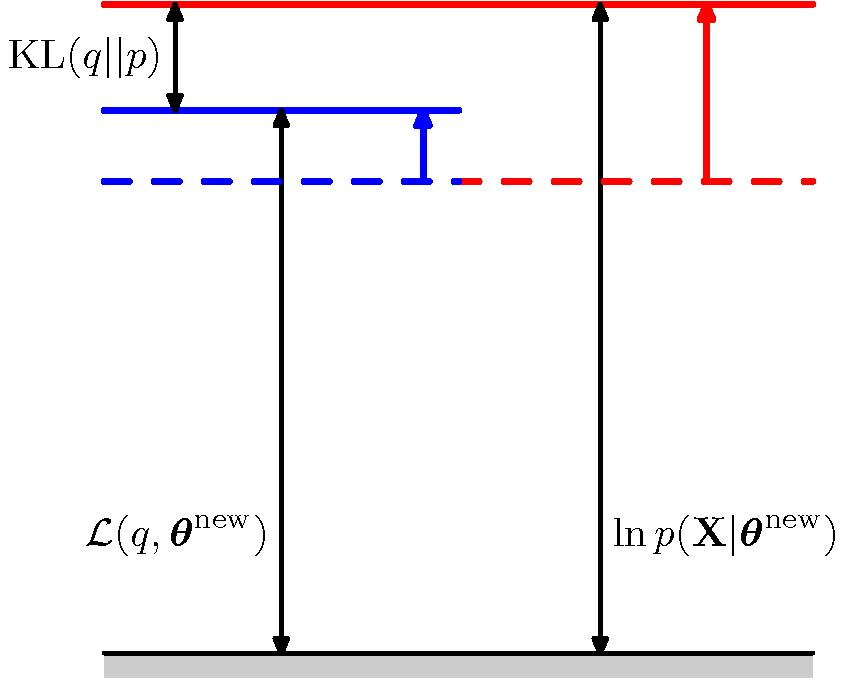
\includegraphics{prml/Figure9.13.jpg}
\end{SCfigure}

Substitute $q(\vec{Z}) = p(\vec{Z}|\vec{X},\vec{\theta}^{old})$ into the lower bound,then after the E step,
\begin{align}
\mathcal{L}(q,\vec{\theta}) 
&= \sum_{\vec{Z}}p(\vec{Z}|\vec{X},\vec{\theta}^{old})\ln p(\vec{X},\vec{Z}|\vec{\theta})
	-\sum_{\vec{Z}}p(\vec{Z}|\vec{X},\vec{\theta}^{old})\ln p(\vec{Z}|\vec{X},\vec{\theta}^{old}) \\
&= \mathcal{Q}(\vec{\theta},\vec{\theta}^{old})	 + const
\end{align}
where the constant is the negative entropy of the $q$ distribution.
\begin{SCfigure*}
	\caption{The EM algorithm involves alternately computing a lower bound on the log likelihood for the current parameter values and then maximizing this bound to obtain the new parameter values.The \color{red} red curve depicts the incomplete-data log likelihood function to maximize.\color{blue} curve where its value equals the log likelihood at $\vec{\theta}^{old}$ indicates the E step.In the M step,the lower bound is maximized giving $\vec{\theta}^{new}$.The \color{green} shows the subsequent E step,constructing a tangential bound at $\vec{\theta}^{new}$ }
	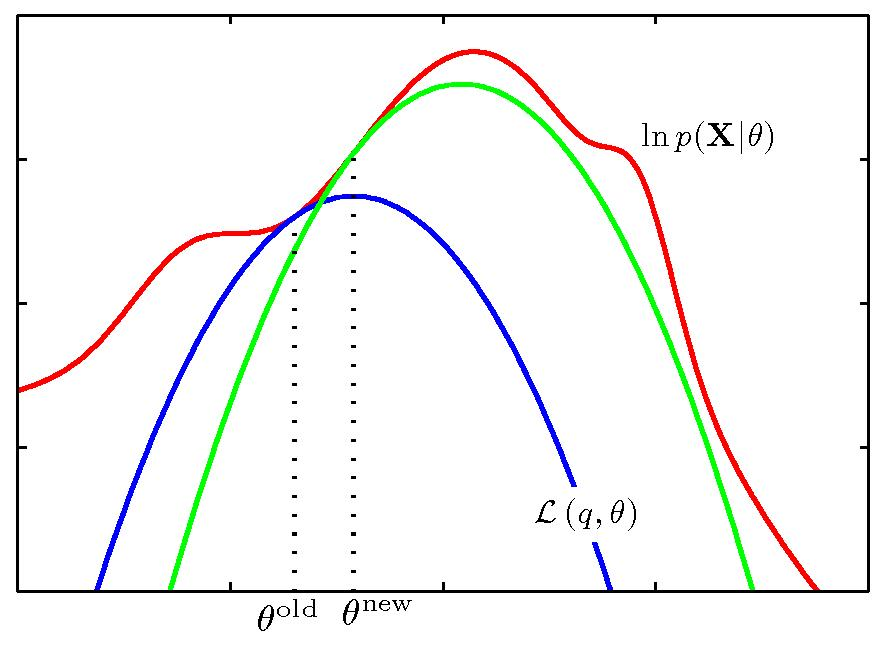
\includegraphics{prml/Figure9.14.jpg}
\end{SCfigure*}

For the particular case of independent,identically distributed data set,$\vec{X}=(\vec{x}_1^T,\vec{x}_2^T,\cdots,\vec{x}_n^T)^T$ and $\vec{Z}=(\vec{z}_1^T,\vec{z}_2^T,\cdots,\vec{z}_n^T)^T$.Using the sum and product rules,the posterior in E step take the form
\begin{align}
p(\vec{Z}|\vec{X},\vec{\theta}) &= \dfrac{p(\vec{X},\vec{Z}|\vec{\theta})}{\sum_{\vec{Z}}p(\vec{X},\vec{Z}|\vec{\theta})}
=\dfrac{\prod_{n=1}^{N}p(\vec{x}_n,\vec{z}_n|\vec{\theta})}{\sum_{\vec{Z}}\prod_{n=1}^{N}p(\vec{x}_n,\vec{z}_n|\vec{\theta})}
=\prod_{n=1}^{N}p(\vec{z}_n|\vec{x}_n,\vec{\theta})
\end{align}
will also factorize with respect to $n$.

\subsection{Maximum posterior}
Maximize the posterior distribution $p(\vec{\theta}|\vec{X})$ with EM for models with a prior $p(\vec{\theta})$ over parameters.
\begin{align}
\because p(\vec{\theta}|\vec{X})&=p(\vec{\theta},\vec{X})/p(\vec{X}) \\
\therefore \ln p(\vec{\theta}|\vec{X})&=\ln p(\vec{\theta},\vec{X})-\ln p(\vec{X})
	=\ln p(\vec{\theta})+\ln p(\vec{X}|\vec{\theta})-\ln p(\vec{X})
\end{align}
decomposed as
\begin{align}
\ln p(\vec{\theta}|\vec{X}) &= \mathcal{L}(q,\vec{\theta})+KL(q\parallel p) +\ln p(\vec{\theta}) -\ln p(\vec{X})\\
&\geq \mathcal{L}(q,\vec{\theta}) +\ln p(\vec{\theta}) -\ln p(\vec{X})
\end{align}
where $\ln p(\vec{X})$ is constant.We can optimize the right-hand side alternatively with respect to $q$ and $\vec{\theta}$ in E-step and M-step.

\subsection{generalized EM}
The \textbf{generalized EM},or GEM,algorithm addresses the problem of an intractable M step.Instead of aiming to maximize $\mathcal{L}(q,\vec{\theta})$ with respect to $\vec{\theta}$,it seeks instead to change the parameters in such a way as to increase its value.
\begin{itemize}
	\item[1]Nonlinear optimization. conjugate gradients algorithm in M step
	\item[2]expectation conditional maximization(ECM). Making several constrained optimizations within each M step.
\end{itemize}

Generalize the E step by performing a \textbf{partial},rather than complete, optimization of $\mathcal{L}(q,\vec{\theta})$ with respect to $q(\vec{Z})$.





